\section{Experiments}
This section evaluates the effectiveness of our proposed \methodfull (\methodtable) with extensive experiments. We aim to address the following research questions: 

\textbf{RQ1.} How does \methodtable perform compared with state-of-the-art models of various types? %Specifically, we compare our model with three types of baselines, including (a) Other graph transformers; (b) Existing neural network models on fixed brain networks; (c) Existing neural network models on learnable brain networks. 

\textbf{RQ2.} How does our proposed \poolingshort module perform with different model choices? 

\textbf{RQ3.} Does the learned model of \methodtable exhibit consistency with existing neuroscience knowledge and suggest reasonable explainability?

\subsection{Experimental Settings}
\label{sec:expset}
\textbf{Datasets.} We conduct experiments on two real-world fMRI datasets. 
(a) \textit{Autism Brain Imaging Data Exchange (ABIDE)}: This dataset collects resting-state functional magnetic resonance imaging (rs-fMRI) data from 17 international sites, and all data are anonymous \citep{abide}. The used dataset contains brain networks from 1009 subjects, with 516 (51.14\%) being Autism spectrum disorder (ASD) patients (positives). The region definition is based on Craddock 200 atlas \cite{craddock2012whole}. As the most convenient open-source large-scale dataset, it provides generated brain networks and can be downloaded directly without permission request. Despite the ease of acquisition, the heterogeneity of the data collection process hinders its use. Since multi-site data are collected from different scanners with different acquisition parameters, non-neural inter-site variability may mask inter-group differences. In practice, we find the training unstable, and there is a significant gap between validation and testing performances. However, we discover that most models can achieve a stable performance if we follow an appropriate stratified sampling strategy by considering collection sites during the training-validation-testing splitting process for ABIDE. Training curves in Appendix \ref{app:setting} also show how different models achieve a stabler performance on our designed new splitting settings than the random splitting. Therefore, we use ABIDE as one of the benchmark datasets in this work, and we share our re-standardized data splitting to provide a fair evaluation pipeline for various future methods.
(b) \textit{Adolescent Brain Cognitive Development Study (ABCD)}: This is one of the largest publicly available fMRI datasets with restricted access (a strict data requesting process needs to be followed to obtain the data) \citep{ABCD}. The data we use in the experiments are fully anonymized brain networks with only biological sex labels. After the quality control process, 7901 subjects are included in the analysis, with 3961 (50.1\%) among them being female. The region definition is based on the HCP 360 ROI atlas \citep{GLASSER2013105}.

\textbf{Metrics.} The diagnosis of ASD is the prediction target on ABIDE, while biological sex prediction is used as the evaluation task for ABCD. Both prediction tasks are binary classification problems, and both datasets are balanced between classes. Hence, AUROC is a proper performance metric adopted for fair comparison at various threshold settings, and accuracy is applied to reflect the prediction performance when the threshold is 0.5. Besides, since the model is mainly for medical applications, we add two critical metrics for diagnostic tests, Sensitivity and Specificity, which respectively refer to true positive rate and true negative rate. All reported performances are the average of 5 random runs on the test set with the standard deviation.

\textbf{Implementation details.} For experiments, we use a two-layer Multi-Head Self-Attention Module and set the number of heads $M$ to 4 for each layer. We randomly split 70\% of the datasets for training, 10\% for validation, and the remaining are utilized as the test set. In the training process of \methodtable, we use an Adam optimizer with an initial learning rate of $10^{-4}$ and a weight decay of $10^{-4}$. The batch size is set as 64. All models are trained for 200 epochs, and the epoch with the highest AUROC performance on the validation set is used for performance comparison on the test set. The model is trained on an NVIDIA Quadro RTX 8000. Please refer to the \href{https://github.com/Wayfear/BrainNetworkTransformer}{repository} and Appendix~\ref{app:software} for the full implementation of \methodtable. 

\textbf{Computation complexity.} In \methodtable, the computation complexity of Multi-Head Self-Attention Module and \poolingshort are $\mathcal{O}(LMV^2)$ and $\mathcal{O}(KV)$ respectively, where $L$ is the layer number of Multi-Head Self-Attention Module, $V$ is the number of nodes, $M$ is the number of heads, and $K$ is the number of clusters in \poolingshort. The overall computation complexity of \methodtable is thus $\mathcal{O}(V^2)$, which is on the same scale as common GNNs on brain networks such as BrainGNN \citep{li2020braingnn} and BrainGB \citep{braingb}. 

\subsection{Performance Analysis (RQ1)}
We compare \methodtable with baselines of three types. The details about how to tune hyperparameters of various baselines can be found in Appendix~\ref{app:turing}. Besides, Appendix~\ref{app:para} shows the comparison of the number of parameters between our model and other baseline models, which shows that the parameter size of \methodtable is larger than GNN and CNN models but smaller than other transformer models.
\textbf{(a) \methodtable vs.~other graph transformers.}
We compare \methodtable with two popular graph Transformers, SAN \citep{san} and Graphormer \citep{graphormer}. In addition, we also include a basic version of \methodtable without \poolingshort, composed of a Transformer with a 2-layer Multi-Head Self-Attention and a CONCAT-based readout named VanillaTF. Our \methodtable outperforms SAN and Graphormer by significant margins, with up to 6\% absolute improvements on both datasets. VanillaTF also surpasses SAN and Graphormer. We believe this downgraded performance of existing graph transformers results from their design flaws facing the natures of brain networks. Specifically, both the preprocessing and the training stages of the Graphormer model accepts only discrete, categorical data. A bin operator has to be applied on the adjacency matrix, coarsening the node feature from connection profiles and dramatically hurting the performance. Furthermore, since brain networks are complete graphs, key designs like centrality encoding and spatial encoding of Graphormer cannot be appropriately applied. Similarly, for SAN, experiments in Appendix \ref{app:node_feature} show that adding eigen node features to connection profiles cannot improve the model's performance. Besides, the benchmark paper~\citep{braingb} reveals that injecting edge weights into the attention mechanism can significantly reduce the prediction power. Furthermore, Appendix~\ref{app:time} shows our \methodtable is much faster than other graph transformers due to special optimizations towards brain networks. \textbf{(b) \methodtable vs.~neural network models on fixed brain networks.}
We further introduce another three neural network baselines on fixed brain networks. BrainGNN~\citep{li2020braingnn} designs ROI-aware GNNs for brain network analysis. BrainGB~\citep{braingb} is a systematic study of how to design effective GNNs for brain network analysis. We adopt their best design as the BrainGB baseline. BrainnetCNN~\citep{BrainNetCNN} represents state-of-the-art of specialized GNNs for brain network analysis, which models the adjacency matrix of a brain network similarly as a 2D image. As is shown in Table \ref{tab:performance}, \methodtable consistently outperforms BrainGNN, BrainGB and BrainnetCNN. \textbf{(c) \methodtable vs.~neural network models on learnable brain networks.} Unlike classical GNNs, FBNETGEN~\citep{kan2022fbnetgen}, DGM~\citep{9763421} and BrainNetGNN~\citep{a14030075} hold a similar idea, which is to apply GNNs based on a learnable graph. FBNETGEN achieves SOTA performance on the ABCD dataset for biological sex prediction, and the learnable graphs can be seen as a type of attention score. Experiment results show that our proposed \methodtable beats all three of them on both datasets.

\begin{table*}[htbp]
\centering
\small
\caption{Performance comparison with different baselines (\%). The performance gains of \methodtable over the baselines have passed the t-test with p-value$<$0.03.}
\label{tab:performance}
\resizebox{1.0\linewidth}{!}{
\begin{tabular}{ccccccccccccc}
\toprule
\multirow{2.5}{*}{Type} & \multirow{2.5}{*}{Method} &\multicolumn{4}{c}{\bf Dataset: ABIDE} & & \multicolumn{4}{c}{\bf Dataset: ABCD}\\
\cmidrule(lr){3-6} \cmidrule(lr){8-11} 
& & {AUROC} & {Accuracy} & {Sensitivity}& {Specificity} & { } & {AUROC} & {Accuracy} & {Sensitivity}& {Specificity} \\
\midrule
\multirow{3}{*}{\thead{Graph\\Transformer}}
& SAN & 71.3±2.1 & 65.3±2.9 & 55.4±9.2& 68.3±7.5 & & 90.1±1.2 & 81.0±1.3 &84.9±3.5&77.5±4.1 \\
& Graphormer & 63.5±3.7 & 60.8±2.7 &\textbf{78.7±22.3}&36.7±23.5 &  & 89.0±1.4 & 80.2±1.3 & 81.8±11.6	&82.4±7.4  \\
& VanillaTF & 76.4±1.2 & 65.2±1.2& 66.4±11.4&71.1±12.0  & &94.3±0.7 & 85.9±1.4& 87.7±2.4&82.6±3.9  \\
\midrule
\multirow{3}{*}{\thead{Fixed\\Network}}
&BrainGNN & 62.4±3.5&59.4±2.3&36.7±24.0&70.7±19.3 && OOM&OOM&OOM&OOM\\
& BrainGB      & 69.7±3.3 & 63.6±1.9& 63.7±8.3&60.4±10.1   & & 91.9±0.3 & 83.1±0.5& 84.6±4.3&81.5±3.9 \\
& BrainNetCNN  & 74.9±2.4 & 67.8±2.7& 63.8±9.7&71.0±10.2   & & 93.5±0.3 & 85.7±0.8& 87.9±3.4&83.0±4.4  \\
\midrule
\multirow{3}{*}{\thead{Learnable\\Network}} 
& FBNETGNN&  75.6±1.2 & 68.0±1.4& 64.7±8.7&62.4±9.2  & & 94.5±0.7 & 87.2±1.2& 87.0±2.5&86.7±2.8   \\
& BrainNetGNN &55.3±1.9&51.2±5.4&67.7±37.5&33.9±34.2 && 75.3±5.2&67.5±4.7&67.7±5.7&68.0±6.5 \\
& DGM & 52.7±3.8&60.7±12.6&53.8±41.2&51.1±40.9 && 76.8±19.0&68.6±8.1&40.5±29.7&\textbf{95.6±4.2} \\
\midrule
\multirow{1}{*}{Ours} 
& \methodtable & \textbf{80.2±1.0} & \textbf{71.0±1.2}& 72.5±5.2&\textbf{69.3±6.5}  & & \textbf{96.2±0.3} & \textbf{88.4±0.4} &\textbf{89.4±2.6}&88.4±1.5 \\
\bottomrule
\end{tabular}
}
\end{table*}

\subsection{Ablation Studies on the \poolingshort Module (RQ2)}

\subsubsection{\poolingshort with varying readout functions}
We vary the readout function for various Transformer architectures, including SAN, Graphormer and VanillaTF, to observe the performance of each ablated model variant. The results shown in Table \ref{tab:readout} demonstrate that our \poolingshort is the most effective readout function for brain networks and improves the prediction power across various Transformer architectures.

\begin{table*}[htbp]
\centering
\small
\caption{Performance comparison AUROC (\%) with different readout functions.}
\label{tab:readout}
\resizebox{0.85\linewidth}{!}{
% add graphomer
\begin{tabular}{cccccccc}
\toprule

\multirow{2.5}{*}{Readout} &\multicolumn{3}{c}{\bf Dataset: ABIDE} & & \multicolumn{3}{c}{\bf Dataset: ABCD}\\
\cmidrule(lr){2-4} \cmidrule(lr){6-8} 
 & {SAN} & {Graphormer}& {VanillaTF} &{ }  & {SAN} & {Graphormer}& {VanillaTF} \\
\midrule
MEAN  & 63.7±2.4 & 50.1±1.1& 73.4±1.4& &88.5±0.9 & 87.6±1.3&91.3±0.7 \\
MAX  & 61.9±2.5 & 54.5±3.6& 75.6±1.4&   & 87.4±1.1 & 81.6±0.8& 94.4±0.6\\
SUM  & 62.0±2.3 & 54.1±1.3& 70.3±1.6&   & 84.2±0.8 & 71.5±0.9& 91.6±0.6\\
SortPooling &68.7±2.3 & 51.3±2.2& 72.4±1.3  &   & 84.6±1.1 & 86.7±1.0& 89.9±0.6\\
DiffPool & 57.4±5.2 &50.5±4.7& 62.9±7.3  &  & 78.1±1.5 & 70.0±1.9& 83.9±1.3 \\
CONCAT & \textbf{71.3±2.1} &63.5±3.7& 76.4±1.2  &  & 90.1±1.2 & 89.0±1.4& 94.3±0.7 \\
\midrule
\poolingshort& 70.6±2.4 &\textbf{64.9±2.7} & \textbf{80.2±1.0} &  & \textbf{91.2±0.7} & \textbf{90.2±0.7}& \textbf{96.2±0.4}\\
\bottomrule
\end{tabular}
}
\end{table*}

\subsubsection{\poolingshort with varying cluster initializations}
To further demonstrate how the design of \poolingshort influences the performance of \methodtable, we investigate two key model selections, the initialization method for cluster centers and the cluster number $K$. For the initialization, three different kinds of initialization procedures are compared, namely (a) \textbf{Random}: the Xavier uniform \citep{glorot2010understanding} is leveraged to randomly generate a group of centers, which are then normalized into unit vectors; (b) \textbf{Learnable}: the same initial process as Random, but the generated centers are further updated with gradient descent; (c) \textbf{Orthonormal}: our proposed process as described in Eq.~\eqref{equ:otho}. 

Specifically, we test each initialization method with the cluster number $K$ equals to {2, 3, 4, 5, 10, 50, 100}. The results of adjusting these two hyper-parameters on ABIDE and ABCD datasets are shown in Figure \ref{fig:parameter}(a). We observe that: (1) When cluster centers are orthonormal, the model's performance increases with the number of clusters ranging from 2 to 10, and then drops with the cluster number rising from 10 to 100, suggesting the optimal cluster number to be relatively small, which leads to less computation and is consistent with the fact that the typical number of functional modules are smaller than 25; (2) With a sufficiently large cluster number, all three initialization methods, Random, Learnable and Orthonormal, tend to reach similar performance, but orthonormal performs stably better when the number of clusters is smaller; (3) It is also notable that our \poolingshort consistently achieves the best performance over other initialization methods regarding smaller standard deviations. 

\begin{figure*}[h]
    \centering
    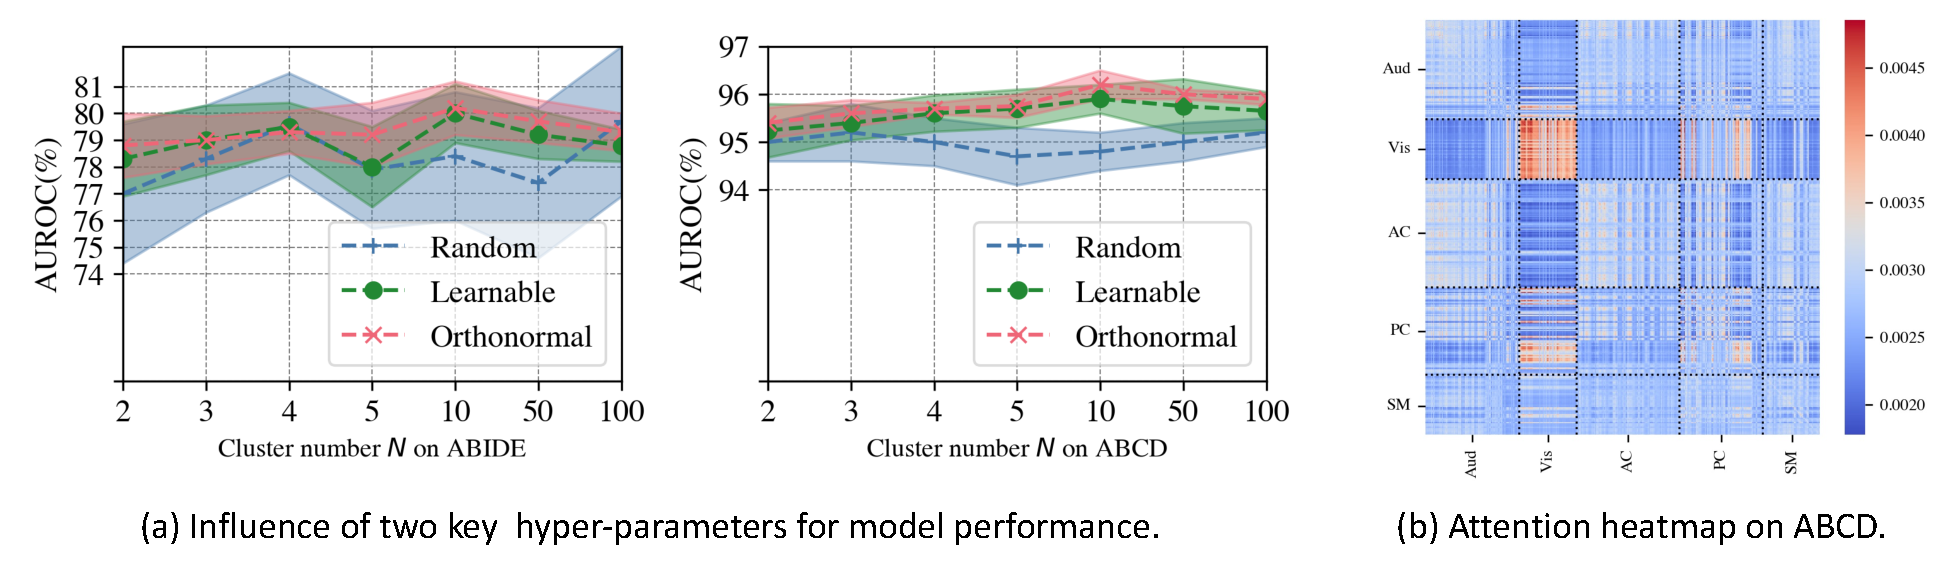
\includegraphics[width=0.90\linewidth]{figures/figure3.pdf}
    \caption{The hyper-parameter influence and the heatmap from self-attention.}
    \label{fig:parameter}
\end{figure*}

\subsection{In-depth Analysis of Attention Scores and Cluster Assignments (RQ3)}
Figure \ref{fig:parameter}(b) displays the self-attention score from the first layer of Multi-Head Self-Attention. The attention scores are the average across all subjects in the ABCD test set. This figure shows that the learned attention scores well match the divisions of functional modules based on available labels, demonstrating the effectiveness and explainability of our Transformer model. Note that since there exists no available functional module labels for the atlas of the ABIDE dataset, we cannot visualize the correlations between attention scores and functional modules.

Figure \ref{fig:soft_att} shows the cluster soft assignment results $\bm P$ on nodes in \poolingshort with two initialization methods. The cluster number $K$ is set to 4. The visualized numerical values are the average $\bm P$ of all subjects in each dataset's test set. From the visualization, we observe that (a) Base on Appendix~\ref{app:difference}, orthonormal initialization produces more discriminative $\bm P$ between classes than random initialization; (b) Within each class, orthonormal initialization encourages the nodes to form groups. These observations demonstrate that our \poolingshort with orthonormal initialization can leverage potential clusters underlying node embeddings, thus automatically grouping brain regions into potential functional modules. 

\begin{figure*}[h]
    \centering
    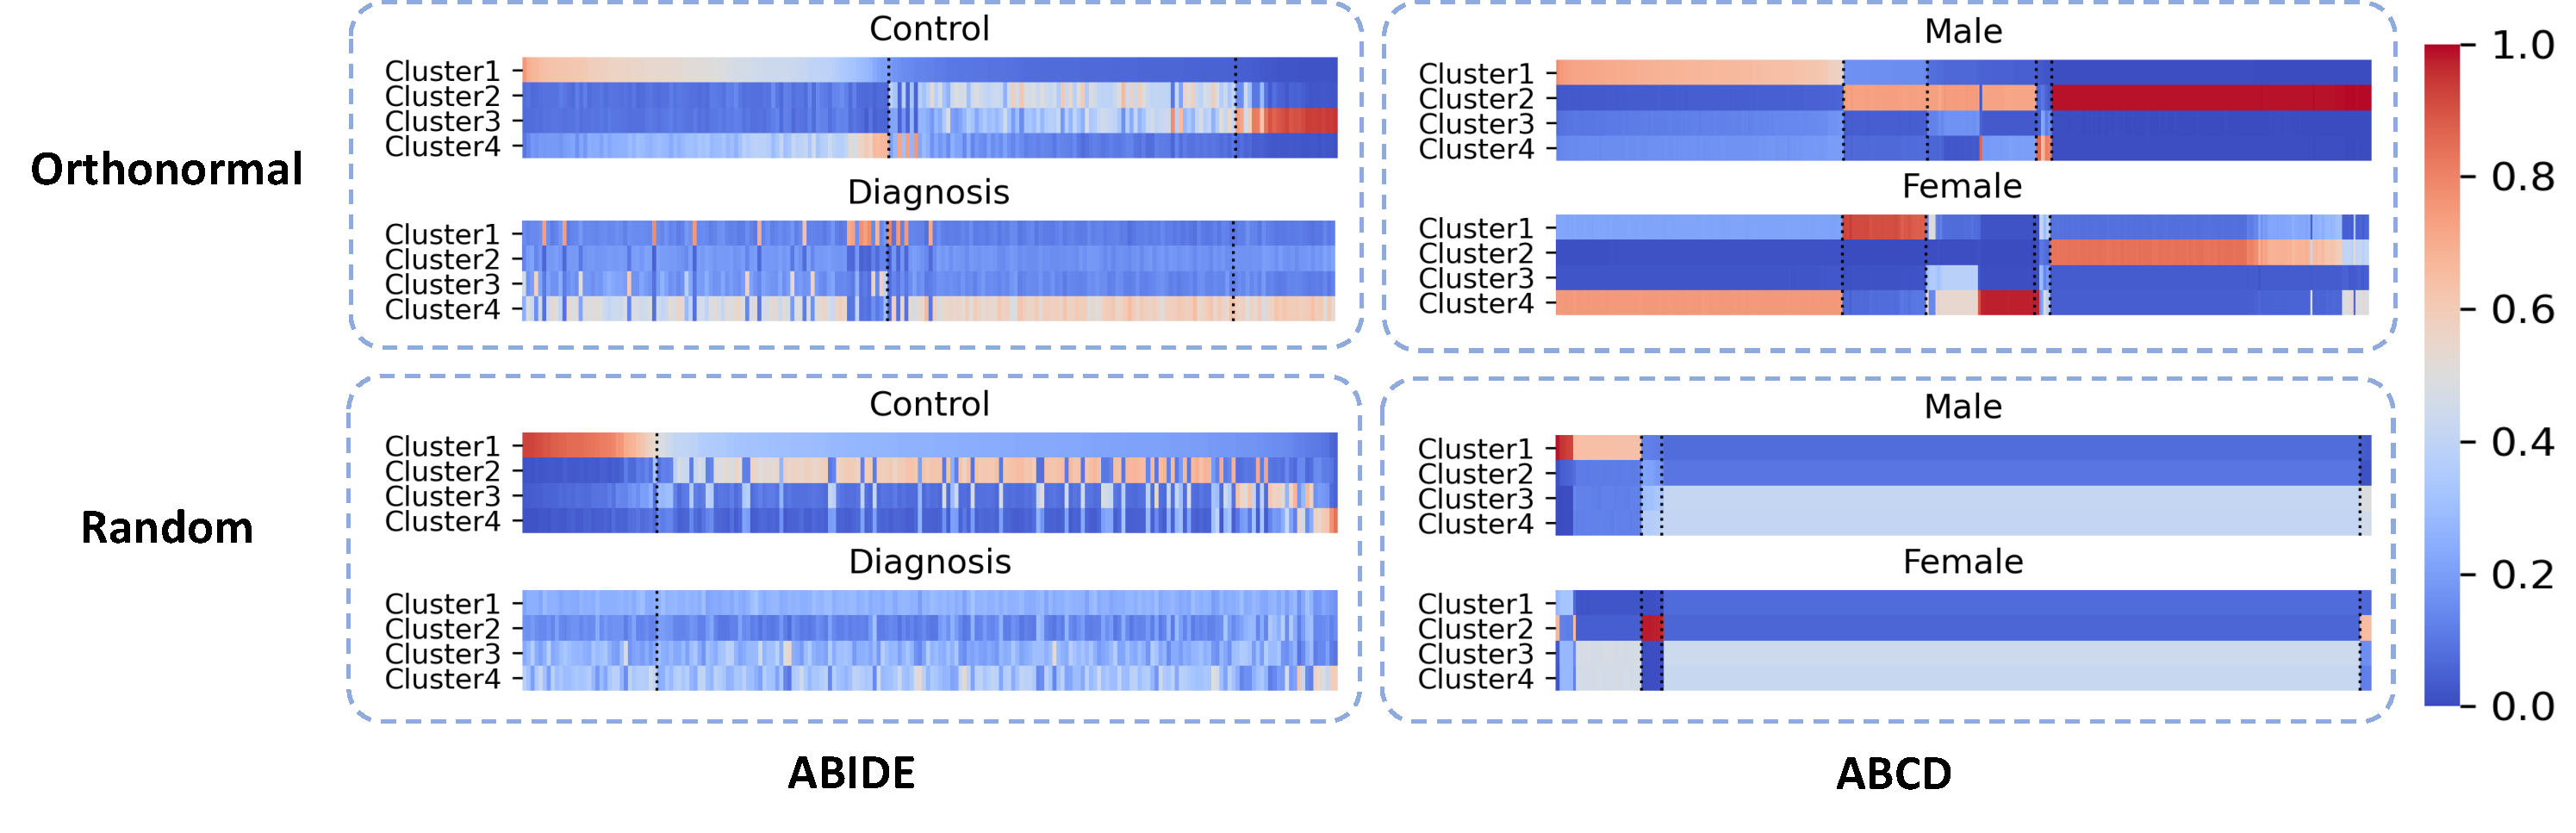
\includegraphics[width=0.9\linewidth]{figures/soft2.pdf}
    \caption{Visualization of cluster (module-level) embeddings learned with Orthonormal vs.~Random cluster center initializations on two datasets.  Each group in the dotted box contains two heatmaps (one for each prediction class) with the same node ordering on the x-axis.}
    \label{fig:soft_att}
\end{figure*}
